\documentclass[tikz]{standalone}
\usepackage{pgfplots}
\pgfplotsset{compat=1.15}
\usepackage{mathrsfs}
\usetikzlibrary{arrows,calc}
\usepackage{tkz-euclide}

\usepackage{fp}
\pagestyle{empty}

\definecolor{AngleClr}{rgb}{0,0.39215686274509803,0}
\definecolor{ShapeClr}{rgb}{0.6,0.2,0}
\definecolor{BlueClr}{RGB}{5,81,163}
\definecolor{GreenClr}{RGB}{7,122,7}

\begin{document}

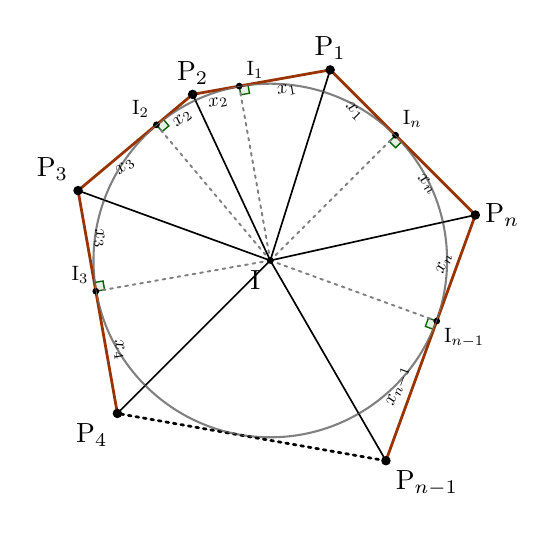
\begin{tikzpicture}[scale=.75]
\tkzSetUpLine[line width=1pt,color=black]
\tkzSetUpPoint[fill=black]

\tkzDefPoints{0/0/I}

% Define the points where the circle touches the quadrilateral.
\tkzDefPoint(45:3){Ia}
\tkzDefPoint(-20:3){Ib}
\tkzDefPoint(-100:3){Ic}
\tkzDefPoint(-170:3){Id}
\tkzDefPoint(130:3){Ie}
\tkzDefPoint(100.1:3){If}

% Find the lines containing the sides of the quadrilateral.
\tkzDefLine[tangent at=Ia](I) \tkzGetPoint{h1}
\tkzDefLine[tangent at=Ib](I) \tkzGetPoint{h2}
\tkzDefLine[tangent at=Ic](I) \tkzGetPoint{h3}
\tkzDefLine[tangent at=Id](I) \tkzGetPoint{h4}
\tkzDefLine[tangent at=Ie](I) \tkzGetPoint{h5}
\tkzDefLine[tangent at=If](I) \tkzGetPoint{h6}


\tkzDrawSegments[line width=0.5pt,color=black,dashed,dash pattern=on 1pt off 1.75pt](I,Ia I,Ib I,Id I,Ie I,If)

% Find the vertices of the quadrilateral.
\tkzInterLL(If,h6)(Ia,h1)\tkzGetPoint{A}
\tkzInterLL(Ia,h1)(Ib,h2)\tkzGetPoint{B}
\tkzInterLL(Ib,h2)(Ic,h3)\tkzGetPoint{C}
\tkzInterLL(Ic,h3)(Id,h4)\tkzGetPoint{D}
\tkzInterLL(Id,h4)(Ie,h5)\tkzGetPoint{E}
\tkzInterLL(Ie,h5)(If,h6)\tkzGetPoint{F}

% Draw the quadrilateral.
\tkzFillPolygon[fill=white](A,B,C,D,E,F)

\tkzMarkRightAngles[line width=0.5pt, size=.15,color=AngleClr,fill=AngleClr,fill opacity=0.1](I,Ia,B I,Ib,C I,Id,E I,Ie,F I,If,A)
\tkzDrawSegments[line width=0.7pt,color=gray,dashed,dash pattern=on 1pt off 1.75pt](I,Ia I,Ib I,Id I,Ie I,If)

\tkzDrawCircle[line width=0.75](I,Ia)

\tkzDrawSegments[color=ShapeClr](A,B E,F F,A D,E B,C)
\tkzDrawSegments[color=black,dashed,dash pattern=on 1pt off 1.75pt](C,D)

\tkzDrawSegments[color=black,line width=0.6pt](I,A I,B I,C I,D I,E I,F)

\tkzDrawPoints[size=3](A,B,C,D,E,F)
\tkzDrawPoints[size=2](Ia,Ib,Id,Ie,If,I)

\tkzDrawCircle(I,Ia)

\tkzLabelPoint[above right,scale=0.75](If){${\rm I}_1$}
\tkzLabelPoint[above right,scale=0.75](Ia){${\rm I}_{n}$}
\tkzLabelPoint[below right,scale=0.75](Ib){${\rm I}_{n-1}$}
% \tkzLabelPoint[below left,scale=0.75](Ic){${\rm I}_4$}
\tkzLabelPoint[above left,scale=0.75](Id){${\rm I}_3$}
\tkzLabelPoint[above left,scale=0.75](Ie){${\rm I}_2$}
\tkzLabelPoint[below left](I){$\rm I$}

\tkzLabelPoint[above](A){${\rm P}_1$}
\tkzLabelPoint[right](B){${\rm P}_{n}$}
\tkzLabelPoint[below right](C){${\rm P}_{n-1}$}
\tkzLabelPoint[below left](D){${\rm P}_{4}$}
\tkzLabelPoint[above left](E){${\rm P}_{3}$}
\tkzLabelPoint[above](F){${\rm P}_2$}

\tkzLabelSegments[below,sloped,scale=0.7](F,If){$x_2$}
\tkzLabelSegments[below,sloped,scale=0.7](F,Ie){$x_2$}

\tkzLabelSegments[below,sloped,scale=0.7](A,If){$x_1$}
\tkzLabelSegments[below,sloped,scale=0.7](A,Ia){$x_1$}

\tkzLabelSegments[below,sloped,scale=0.7](B,Ia){$x_{n}$}
\tkzLabelSegments[above,sloped,scale=0.7](B,Ib){$x_{n}$}

\tkzLabelSegments[above,sloped,scale=0.7](C,Ib){$x_{n-1}$}
% \tkzLabelSegments[above,sloped,scale=0.7](C,Ic){$x_4$}

% \tkzLabelSegments[above,sloped,scale=0.7](D,Ic){$x_{2n-1}$}
\tkzLabelSegments[above,sloped,scale=0.7](D,Id){$x_{4}$}

\tkzLabelSegments[above,sloped,scale=0.7](E,Id){$x_3$}
\tkzLabelSegments[below,sloped,scale=0.7](E,Ie){$x_3$}


\end{tikzpicture}

\end{document}
